% LLNCStmpl.tex
% Template file to use for LLNCS papers prepared in LaTeX
%websites for more information: http://www.springer.com
%http://www.springer.com/lncs

\documentclass{llncs}
%Use this line instead if you want to use running heads (i.e. headers on each page):
%\documentclass[runningheads]{llncs}
\usepackage[english]{babel}
\usepackage[utf8]{inputenc}
\usepackage{multimedia}
\usepackage{mathtools}
\usepackage{paratype}
\usepackage{float}
\usepackage{graphicx}
\usepackage{caption}
\usepackage{subcaption}
\captionsetup{compatibility=false}

\begin{document}
\title{DSSS and FHSS}

%If you're using runningheads you can add an abreviated title for the running head on odd pages using the following
%\titlerunning{abreviated title goes here}
%and an alternative title for the table of contents:
%\toctitle{table of contents title}

\subtitle{A comparison of two modulation schemes}

%For a single author
%\author{Author Name}

%For multiple authors:
\author{Group 6: Urs Gerber, Gian-Luca Mateo, Niclas Scheuing, Roger Stebler} 


%If using runnningheads you can abbreviate the author name on even pages:
%\authorrunning{abbreviated author name}
%and you can change the author name in the table of contents
%\tocauthor{enhanced author name}

%For a single institute
%\institute{Institute Name \email{email address}}

% If authors are from different institutes 
\institute{University of Berne \email{email address}}

%to remove your email just remove '\email{email address}'
% you can also remove the thanks footnote by removing '\thanks{Thank you to...}'


\maketitle

%\begin{abstract}
%abstract text goes here - Lorem ipsum dolor sit amet, consectetur adipiscing elit, sed do eiusmod tempor incididunt ut labore et dolore magna aliqua.
%\end{abstract}

\section{Protocol Introduction}
\label{sec:theory}
	\emph{Spread  Spectrum} is a procedure to spread a transmission over a wider frequency range. The goal is robustness and support for parallel transmissions.
	Refer to \cite{ISS} for more details.
	
	Both, \emph{FHSS} and \emph{DSSS} require the sender and receiver to be time-synchronized. 
	
	\subsection{Frequency Hopping Spread Spectrum}
		In \emph{FHSS} the frequency band $f$ is split into $N$ sub-bands $f_1,..., f_N$. Each sender gets a pseudo-random chip sequence $p_n \in [f_1,...,f_N]^n$ which is known by the sender and the receiver only.
		
		\paragraph{Slow hopping} The sender will start by taking the first sub-band from its chip sequence $p_n$ and transmit on this sub-band.
		After a defined dwell time, it takes the next sub-band from $p_n$ and continue this procedure. The dwell time $T_h$ is a multiple of the symbol time $T_s$. $T_s$ is the time during which one symbol is broadcast.
		
		\paragraph{Fast hopping} In this case the symbol time $T_s$ is a multiple of the dwell time $T_h$. During the transmission of one symbol, one or multiple hops are made. So one symbol is transmitted on multiple frequencies.
		
		\paragraph{Interference} FHSS is very robust under narrow-band interference. If one sub-channel is jammed, this will only affect part of the transmission. Any other user using the same FHSS scheme will appear as narrow-band interference.
		Broad-band interference can not be easily dealt with.
		
	
	\subsection{Direct Sequence Spread Spectrum}
		Each sender has a chip sequence $p_n \in \{-1,1\}^n, \sum p_n = 1$ known the sender and receiver only. The chip-rate $R_c$ is a multiple of the signal-rate $R_s$.
		
		\paragraph{Spreading} Before sending the data sequence $d_t$, it is multiplied point-wise with the chip-pattern resulting in the transmission data $t_x = d_t p_n$.
		Image \ref{dsss} shows an example of these steps.
		This multiplication is called \emph{spreading} because the frequency of the original data $R_s$ has been increased to the frequency of the chip pattern $R_c$. This can be seen on the right side of Figure \ref{dsss}.
		
		\paragraph{Despreading} is the inverse of the spreading operation. The received signal $r_x$ is again point-wise multiplied with the chip pattern resulting in the despread data. Since $p_n p_n = [1,...,1]$, this will return the original data $d_r = t_x p_n = d_t p_n p_n = d_t$.
		
		\paragraph{Chip pattern} The length of the chip pattern $T_c$ is either the symbol length $T_s$ (short code) or a multiple of the $T_s$ (long code).
		
		When multiple users are transmitting on the same frequency range, their pattern have to be orthogonal.
		
		\paragraph{Interference} Narrow-band interference will be spread during the despreading and have little impact on the SNR. Broad-band signals uncorrelated to the chip pattern will not be affected by the despreading and thus have a higher impact on the SNR.
		See Figure \ref{dsss_interference}.
\section{Experiment Setup}

	In the following sections we introduce the general experiment setup as well as the various test scenarios and parameters that were used to obtain the final results.
	
	\subsection{Test Architecture}
	Our simulation of the spread spectrum mechanisms is based on a simple pipeline, where a \emph{sender} is writing its data onto a \emph{medium}. Various kinds of interference is generated by a \emph{jammer} which adds its data to the same medium. Finally the \emph{receiver} reads data from the medium and tries to decode the original bit sequence.
	
	\paragraph{Sender}
	The sender is responsible for spreading a random data sequence consisting of $0$s and $1$s using either the \emph{DSSS} or \emph{FHSS} spreading mechanism as explained in section \ref{sec:theory}. After spreading, the sender will modulate the spread data onto passband using the BPSK modulation scheme (using a phase-shift of $\Delta \phi = \pi / 2$) with a carrier frequency $f_c$ in the case of DSSS. With FHSS, the sender generates a set of $N=8$ sub-carrier frequency bands of bandwidth $\Delta f$. The modulated signal is then passed to the \emph{medium}
	
	\paragraph{Medium} 
	After a signal is sent to the medium, we perform a Fast Fourier Transform (FFT) of the data and store the result. A jammer may then add an interference signal onto the original data, depending on the respective test scenario. Whenever a receiver reads data from the medium, we perform an inverse FFT and pass the data to the receiver.
	
	\paragraph{Receiver}
	The receiver first reads the data off the medium and applies the respective demodulation scheme according to the scheme that was used to send the data in the first place. If DSSS was used, the receiver simply demodulates the whole signal using BPSK and despreads the signal using the same pn-sequence that the sender used. In the case of FHSS the receiver splits the data into slices equal in length to a chip -- depending on the channel number determined by the pn-sequence. Each chip is then demodulated using BPSK and decoded. 
		
	\paragraph{Jammer}
	We used multiple approaches to designing our jammer. The most reliable method -- the method we used in our results -- was designing the jammer as just another DSSS user whose bandwidth we can control using the chipping rate. One of the most difficult aspects of this simulation was the power control of this jammer with respect to the signal power that is already on the medium. As a result, we always specify the power of the jammer as a power factor $p_f$ relative to the total power of the signal to be jammed.
	
	\subsection{Testing Scenarios and Parameters}
	The used test metric was solely the relative bit error rate $BER$. This was computed as the number of bit errors per sent data sequence $BE$ divided by the length of the data sequence.
	
	\[
		BER = \frac{BE}{length(data)}
	\]
	
	Each test was repeated $20$ times, yielding an effective average over all test runs.
	
	Throughout all test scenarios, the carrier frequency for all DSSS tests remained $f_c = 100\text{Hz}$. The channel configuration for FHSS is also constant, with the $N=8$ sub-carriers starting at frequency $f_c = 100\text{Hz}$ with a channel bandwidth of $\Delta f = 128 \text{Hz}$, resulting in sub-carriers at $f_i = (100 + i \cdot 128)\text{Hz}, i=1,..,N$ The symbol rate was fixed at $f_{sym} = 8\text{Hz}$. In each test, white Gaussian noise with an SNR of $10\text{dB}$ was added to the time domain signal to simulate interference of various origins.
	
	Each test scenario was conducted with the same variable parameters consisting of the chipping rate $f_{chip}$ and the length of the pn-sequence $l_{pn}$. For both FHSS and DSSS, we used $l_{pn} = (16, 64)$. Initial tests showed that these are sensible values. The chipping rates used in DSSS were $f_{chip}^{DSSS} = (16,32,64,96)\text{Hz}$, in FHSS $f_{chip}^{FHSS} = (1, 4, 16, 32)$ respectively. Combined, the two paremeter sets $l_{pn}$ and $f_{chip}$ form eight curves in each plot of a test scenario.
	
	\paragraph{Narrowband Interference}
	In this scenario we tested the performance of both spreading schemes under the influence of narrowband interference. For DSSS, we jammed the $f_{jam} = 100\text{Hz}$ carrier with a noise bandwidth of $\Delta f_{jam} = 8\text{Hz}$ at various noise power factors $p_f$ from $0$ to $7$ in $0.5$ step increments. For FHSS, we successively jammed each sub-carrier channel, from $0$ to all $8$ channels with a noise bandwidth of $\Delta f_{jam} = 64\text{Hz}$, as we wanted to jam a whole sub-carrier channel. The power factor for each jam channel was set to $p_f = 2.5$.
	
	\paragraph{Wideband Interference}
	Wideband interference is the core weakness of both spread specrum techniques -- a fact that we wanted to simulate. The DSSS test run was conducted using a jamming bandwidth of $\Delta f_{jam} = 200\text{Hz}$ again targeted at $f_{jam} = 100\text{Hz}$. The jamming power factor was scaled from $1$ to $15$ to simulate various strengths of wideband interference. For FHSS, a noise bandwidth of $\Delta f_{jam} = 1000\text{Hz}$  was used and the jammed frequency was moved close to the center of the sub-carriers $f_{jam} = 550\text{Hz}$. The noise power factor was scaled from $2$ to $4$ in $0.5$ increments. We expected both schemes to handle wideband interference equally bad.
	
	\paragraph{Varying Noise Bandwidth}	
	An interesting scenario represents the performance of the spreading schemes in presence of various noise bandwidths. With our jammer design, this kind of comparison was very hard to achieve since a change in bandwidth also meant a change in power. We had to also adapt the power factor for each tested bandwidth to obtain comparable results. For both DSSS and FHSS we used $\Delta f_{fam} = (8,16,32,64,128,256)\text{Hz}$ with a matching power factor $p_f = (1,2,2.5,3,3.5,4)$. These power factors were obtained by visually matching in all conscience the noise power density to figures given in \cite{ISS} and are by no means exact. The jammed frequency was $f_{jam}=100\text{Hz}$ for both schemes. 
	
	\paragraph{Multiple Users}
	In this scenario we tested how well DSSS and FHSS handle multiple users on the same frequency band. In both cases, we scaled the number of users from $1$ to $15$. We expected FHSS to handle this situation better than DSSS, since additional FHSS users appear as narrowband interference. The sender power for each user was kept the same.
	
	\paragraph{Varying strength of white Gaussian noise}
	In this last scenario we tested the performance of DSSS and FHSS in presence of average white Gaussian noise of various strengths. The SNR was scaled from $-2\text{dB}$ to $-10\text{dB}$ in the case of FHSS and from $-8\text{dB}$ to $-30\text{dB}$ for DSSS. We did not expect any scheme to perform substantially better.
	
	
	
\section{Results and Analysis}
	Using the test setup and cases shown above, we were able to gain the following insights.
	\subsection{DSSS}
		\subsubsection{Performance in presence of narrowband and wideband interference}~\\
			Figure \ref{fig:dsss_narrowband} shows error rate of DSSS under narrowband noise. We observe that higher \emph{chipping rates} - which lead to broader spreading - add robustness.
			This is due to the narrowband interference getting despread more strongly when employing higher chipping rates.
			The \emph{chip sequence length} has little to no influence, which also matches our expectations, as the power spectrum does not change with different chip length. longer chip sequences do, hovewer, add support for more users.
			
			Figure \ref{fig:dsss_wideband} illustrates behaviour under the influence of wideband noise, which is nearly identical for all our different testing parameters.
			We would intuitively have expected low \emph{chipping rates} to have better performance - due to their more narrow frequency spectrum and thus higher peak power - but this line of thought ignores that wideband noise is not correllated with the sent signal, and so does not get despread. Thus, it remains on the same power level after despreading, which results in the invariability of performance under changing parameters.
			
			Due to our testing setup and methodology, direct comparison between the two scenarios is tedious. As our jammer implementation puts out a constant base power when measuring over the whole spectrum, the SNRs tend to be very different for different scenarios. Because of that, we have chosen to regard narrowband and wideband noise as separate cases and do a comparison in a separate test case, where we tried to visually match the signal and noise spectra of the scenarios outlined in \cite{ISS}. The results of that test are shown in \ref{fig:dsss_bandwidth} and discussed in the next section.
				\begin{figure}[H]
					\centering
					\caption{}
				    \begin{subfigure}[b]{0.5\textwidth}
						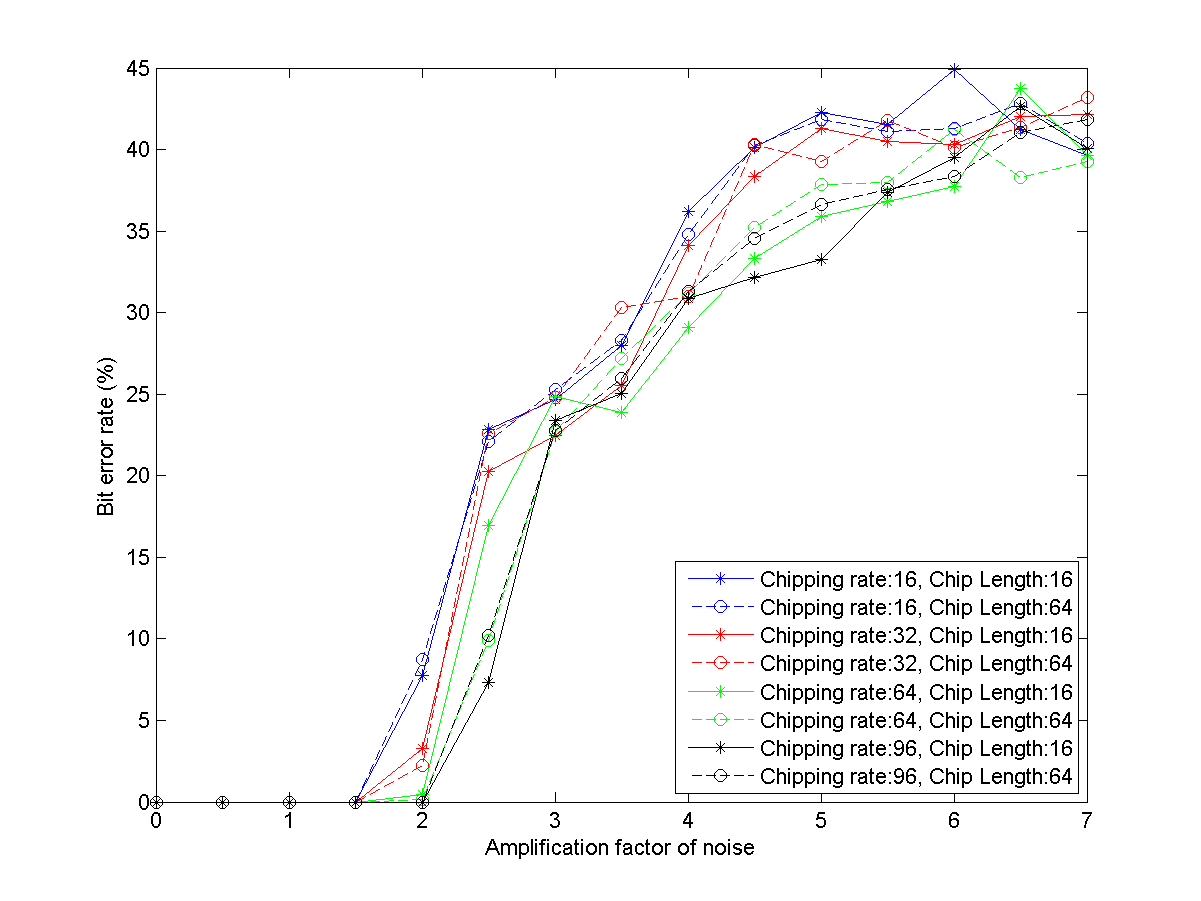
\includegraphics[width=\textwidth]{imgs/results/plot_mode_dsss-test_narrowband-rep_20-dataRate_8-dataLength_128.png}
						\caption{DSSS Narrowband noise: $\Delta f= 8 \text{Hz}, f_{jam} = 100\text{Hz}$}
						\label{fig:dsss_narrowband}
					\end{subfigure}%
					~
					\begin{subfigure}[b]{0.5\textwidth}
						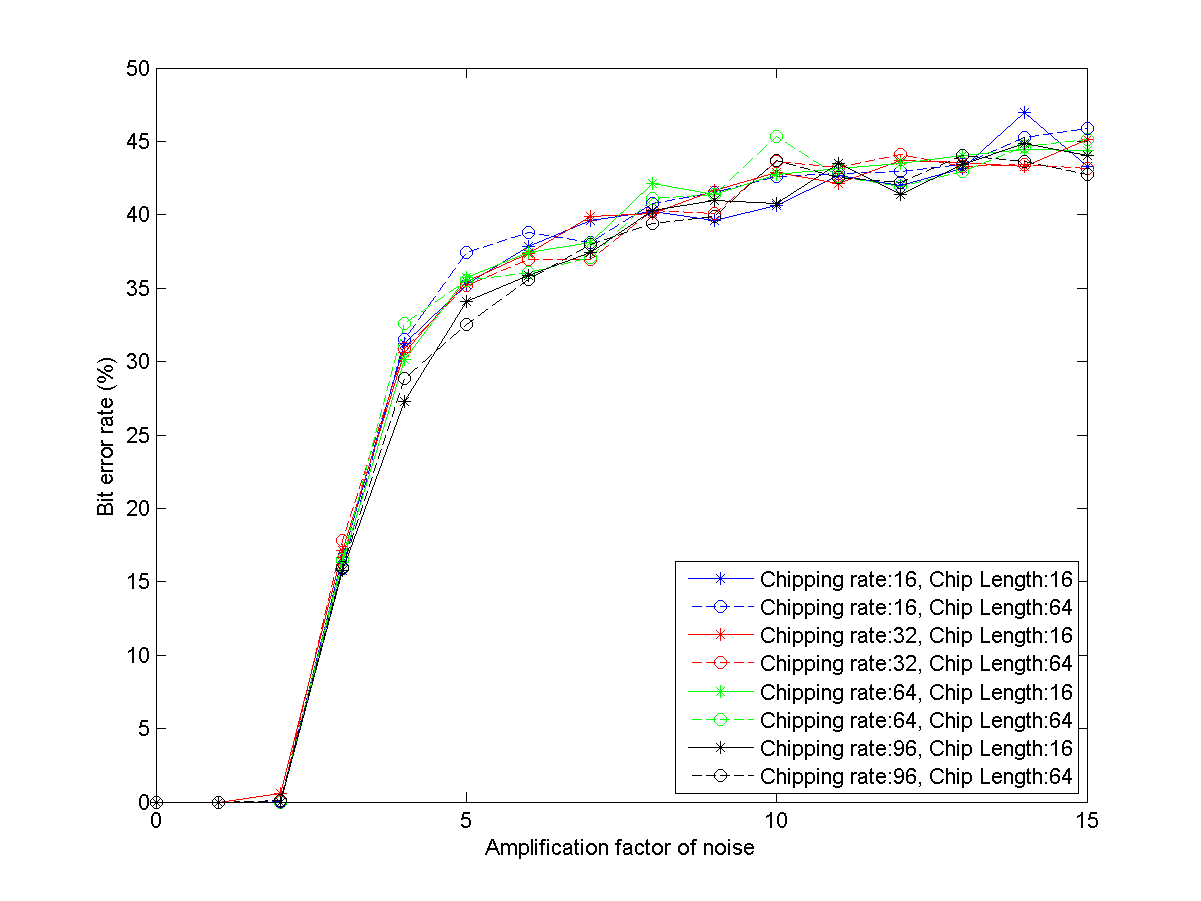
\includegraphics[width=\textwidth]{imgs/results/plot_mode_dsss-test_wideband-rep_20-dataRate_8-dataLength_128.png}
						\caption{DSSS Wideband noise: $\Delta f = 200 \text{Hz}, f_{jam} = 100\text{Hz}$}
						\label{fig:dsss_wideband}
					\end{subfigure}
				\end{figure}
				
		
		\subsubsection{Performance with varying interference bandwidth and white Gaussian noise}\label{sec:real-life}~\\
			Figure \ref{fig:dsss_bandwidth} shows the results of the aforementioned test case.
			\emph{Wideband noise} has a bigger impact on performance than \emph{narrowband noise} with high \emph{chipping rates} showing better performance than low ones.
			While we are very aware that the parameters for this configuration may seem arbitrary, we struggled to find reliable reference values. The result of this is that the results should be seen as a qualitative estimation of real-world performance of DSSS under presumably realistic levels and bandwidths of interference and not as exact values. 
			
			Figure \ref{fig:dsss_gaussian} outlines performance of our DSSS implementation with varying levels of white Gaussian noise.
			The results widely match expected behaviour, with performance deteriorating with more added noise.
			Unexpectedly, performance was worse when employing low chipping rates.
			We suspect this may be due to the way MATLAB measures the SNR when using the \emph{awgn} function.
			
			\begin{figure}[H]
				\centering
				\caption{}
				\begin{subfigure}[b]{0.5\textwidth}
					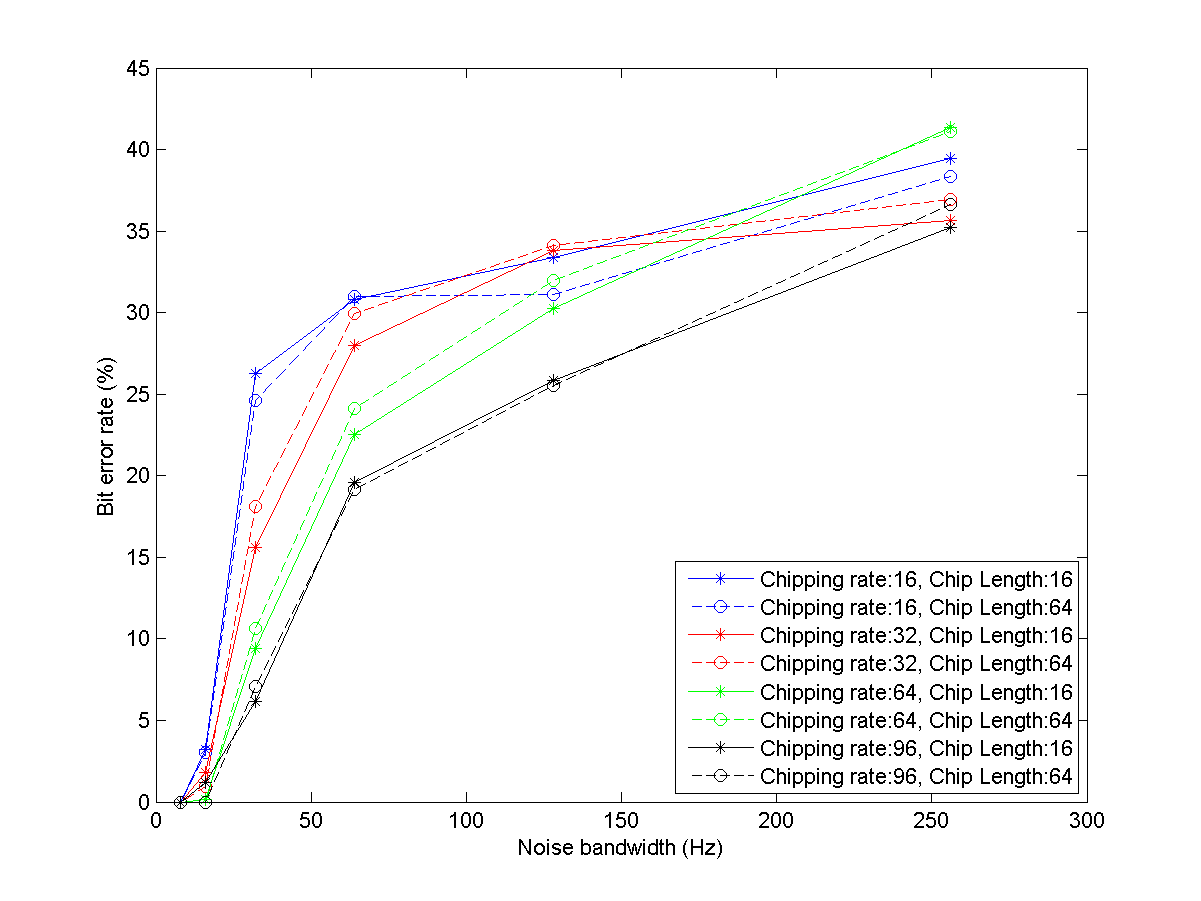
\includegraphics[width=\textwidth]{imgs/results/plot_mode_dsss-test_bandwidthAndPower-rep_20-dataRate_8-dataLength_128.png}
					\caption{DSSS: Various noise bandwidths and powers: $p_f = (1,2,2.5,3,3.5,4)$}
					\label{fig:dsss_bandwidth}
				\end{subfigure}%
				~
				\begin{subfigure}[b]{0.5\textwidth}
					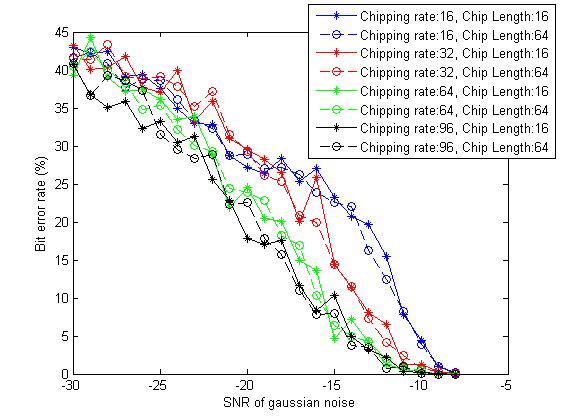
\includegraphics[width=\textwidth]{imgs/results/plot_mode_dsss-test_gaussianSNR-rep_20-dataRate_8-dataLength_128_fixedlegend.png}
					\caption{DSSS: Various SNR of white Gaussian noise}
					\label{fig:dsss_gaussian}
				\end{subfigure}
			\end{figure}		
				
		\subsubsection{Performance with multiple users}~\\
				
			In Figure \ref{fig:dsss_multiuser} we see that low \emph{chipping rates} work considerably worse than high chipping rates, as the signal is spread less.
			This matches expected behaviour.
				
			\begin{figure}[H]
			\centering
				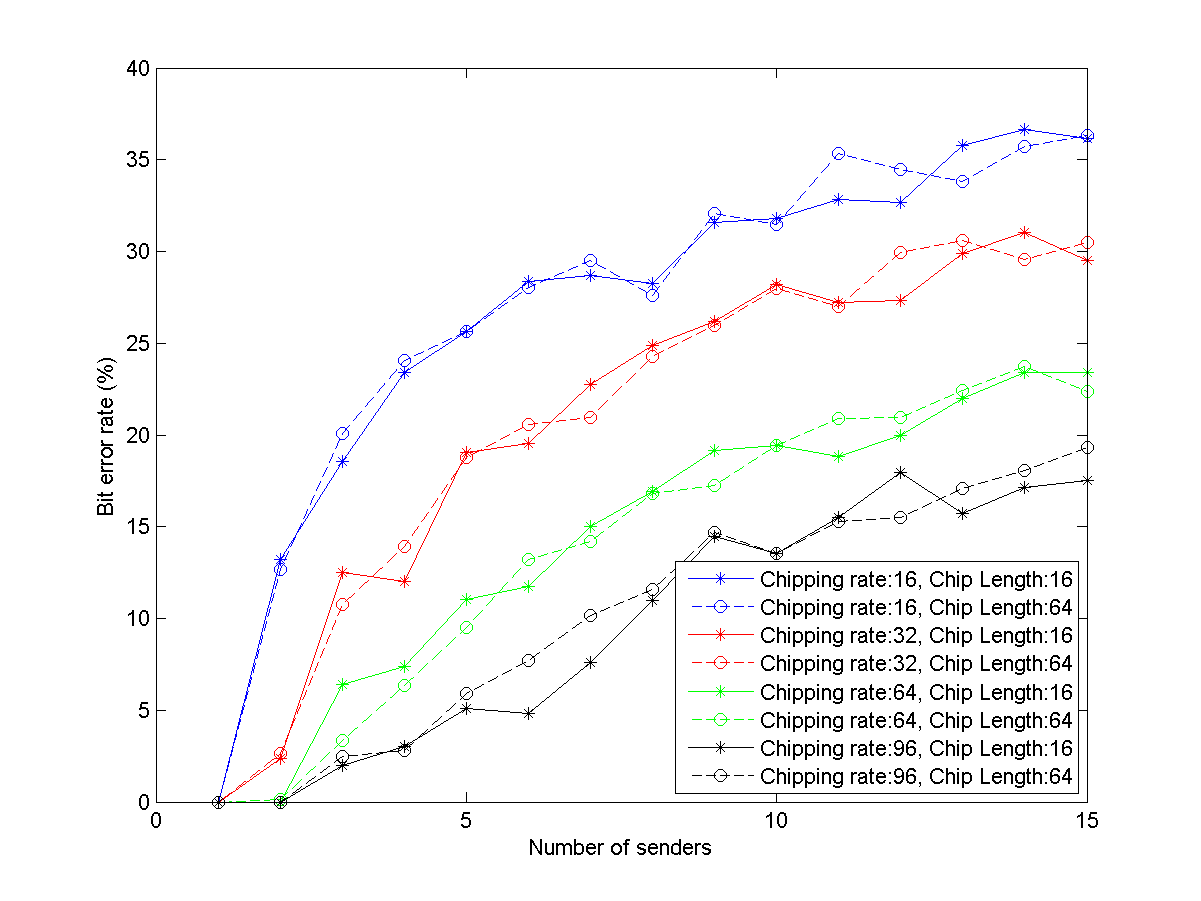
\includegraphics[width=0.5\textwidth]{imgs/results/plot_mode_dsss-test_numSenders-rep_20-dataRate_8-dataLength_128.png}
				\caption{DSSS: Multiuser}
				\label{fig:dsss_multiuser}
			\end{figure}
	
	\subsection{FHSS}
		
		Before going into the exact test cases, it is important to note that there is a problem with our implementation of fast frequency hopping, as it works badly with BPSK modulation. Various websites such as \cite{web-nl} emphasize the difficulty of using coherent data detection and that FSK is most often used. However, we followed our requirements and implemented BPSK.
		
		\subsubsection{Performance in presence of narrowband and wideband interference}~\\
			The results widely match expected behaviour, with performance deteriorating the more channels are jammed and wideband noise affecting all channels - and thus all configurations - equally.
			Importantly, we were not able to create configurations where without crosstalk between the different channels, so this will have influenced all results.
			
			\begin{figure}[H]
				\centering
				\caption{}
				\begin{subfigure}[b]{0.5\textwidth}
					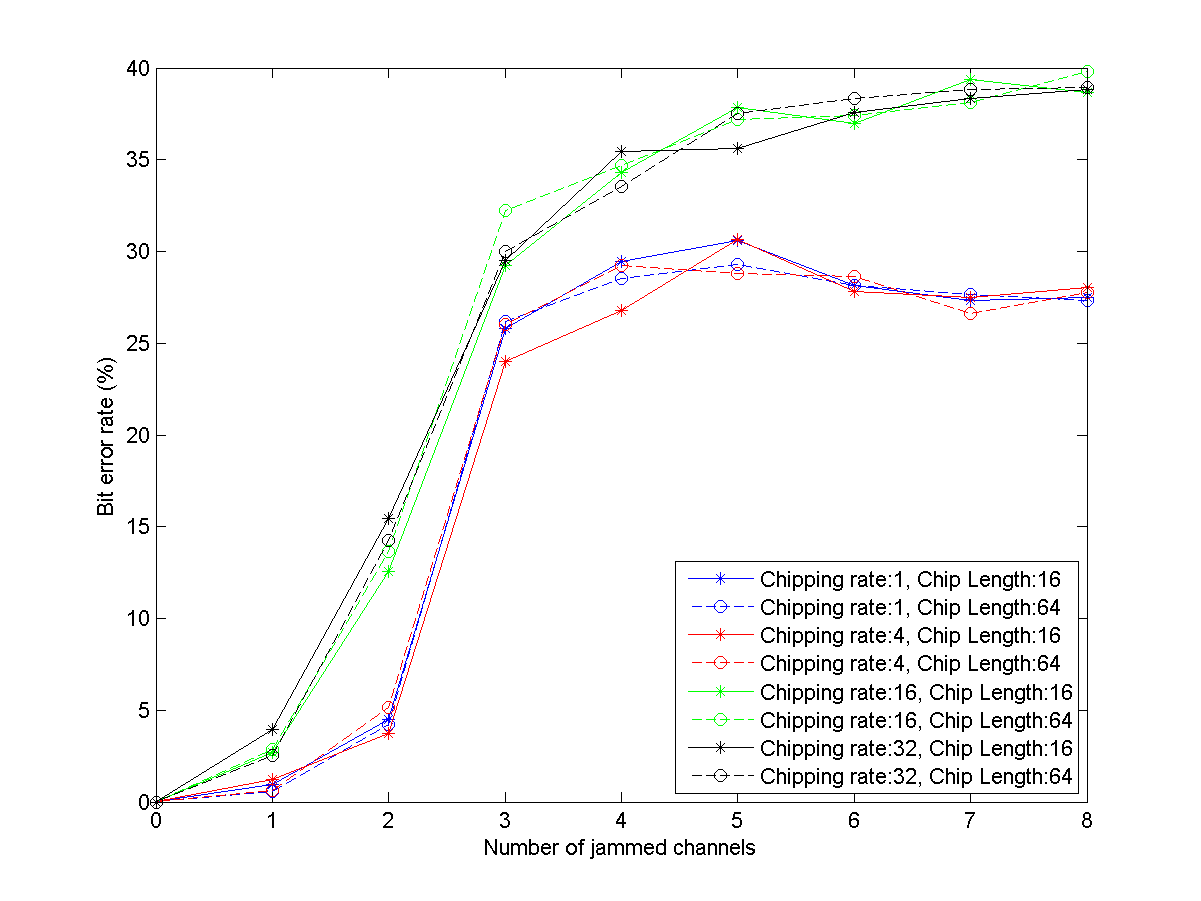
\includegraphics[width=\textwidth]{imgs/results/plot_mode_fhss-test_narrowband-rep_20-dataRate_8-dataLength_128.png}
					\caption{FHSS: Narrowband noise: $\Delta f= 64 \text{Hz}, p_f = 2.5$}
					\label{fig:fhss_narrowband}
				\end{subfigure}%
				~
				\begin{subfigure}[b]{0.5\textwidth}
					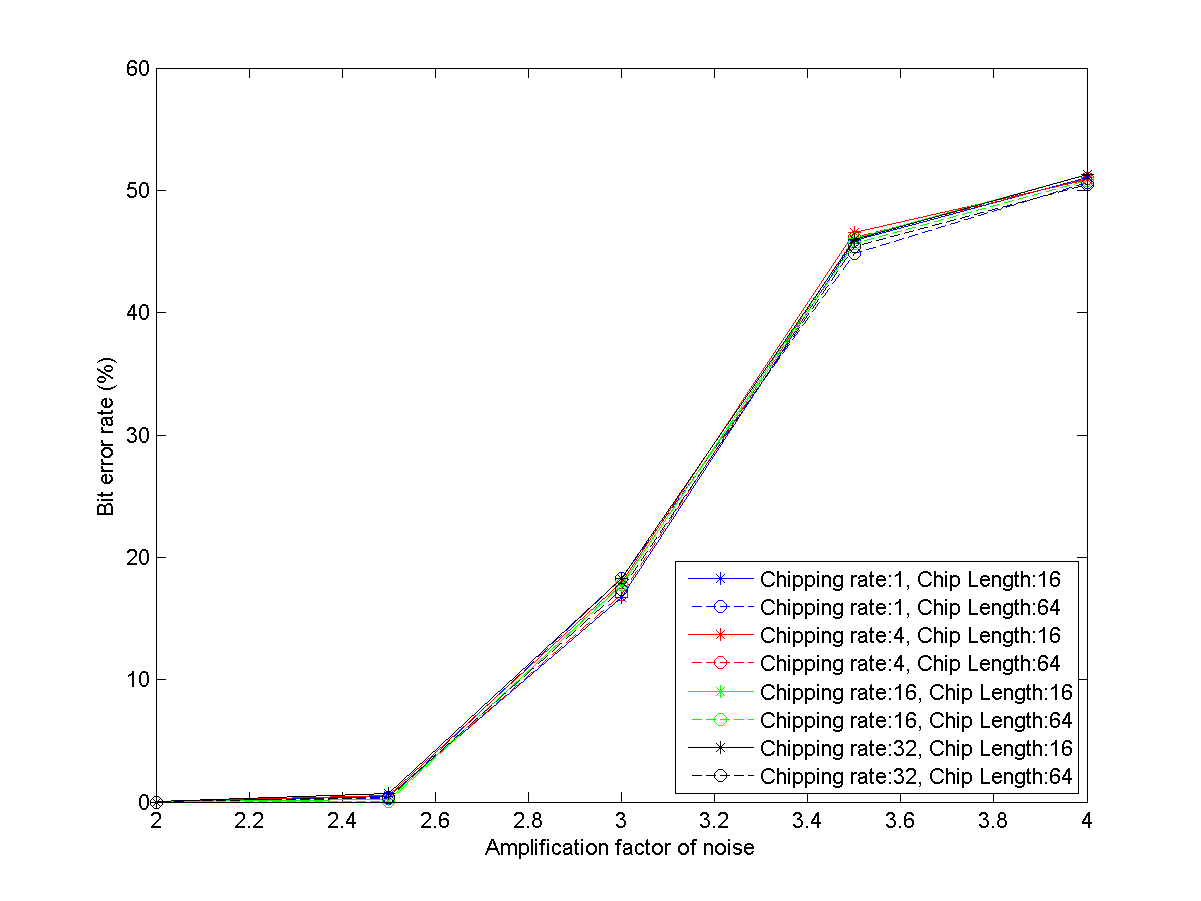
\includegraphics[width=\textwidth]{imgs/results/plot_mode_fhss-test_wideband-rep_20-dataRate_8-dataLength_128.png}
					\caption{FHSS: Wideband noise: $\Delta f= 200 \text{Hz}, f_{jam} = 550\text{Hz}$}
					\label{fig:fhss_wideband}
				\end{subfigure}
			\end{figure}
			
			
		\subsubsection{Performance with varying interference bandwidth and white Gaussian noise}~\\
			The results shown in Figure \ref{fig:fhss_bandwidth} again represent an estimation of performance under different - and presumably realistic - noise configurations.
			The results are similar to the ones from DSSS, with better performance under the influence of narrowband interference.
			Figure \ref{fig:fhss_gaussian} shows a more streamlined result than DSSS, which is caused by the bandwidths and channel configurations being invariable under the different parameter configurations.
	
			\begin{figure}[H]
				\centering
				\caption{}
				\begin{subfigure}[b]{0.5\textwidth}
					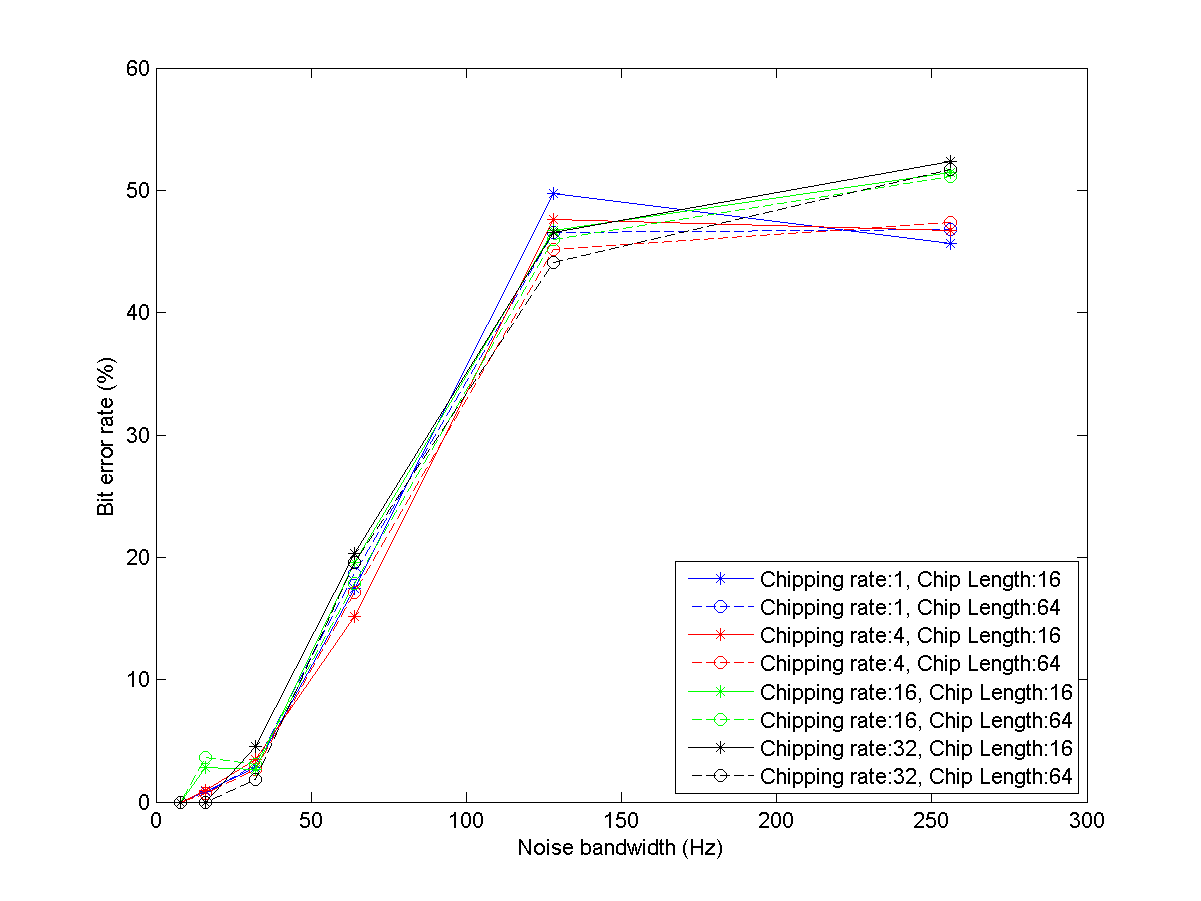
\includegraphics[width=\textwidth]{imgs/results/plot_mode_fhss-test_bandwidthAndPower-rep_20-dataRate_8-dataLength_128.png}
					\caption{FHSS: Various noise bandwidth and power: $p_f = (1,2,2.5,3,3.5,4)$}
					\label{fig:fhss_bandwidth}
				\end{subfigure}%
				~
				\begin{subfigure}[b]{0.5\textwidth}
					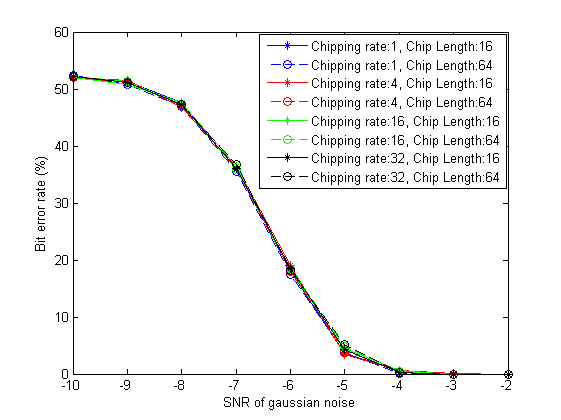
\includegraphics[width=\textwidth]{imgs/results/plot_mode_fhss-test_gaussianSNR-rep_20-dataRate_8-dataLength_128_fixedlegend.png}
					\caption{FHSS: Various SNR of white Gaussian Noise}
					\label{fig:fhss_gaussian}
				\end{subfigure}
			\end{figure}
		
		\subsubsection{Performance with multiple users}~\\
			The results shown match expected behaviour. The performance deteriorates quickly and bottoms at 40-50 \% BER when the number of users approaches the number of channels.
			
			\begin{figure}[H]
			\centering
				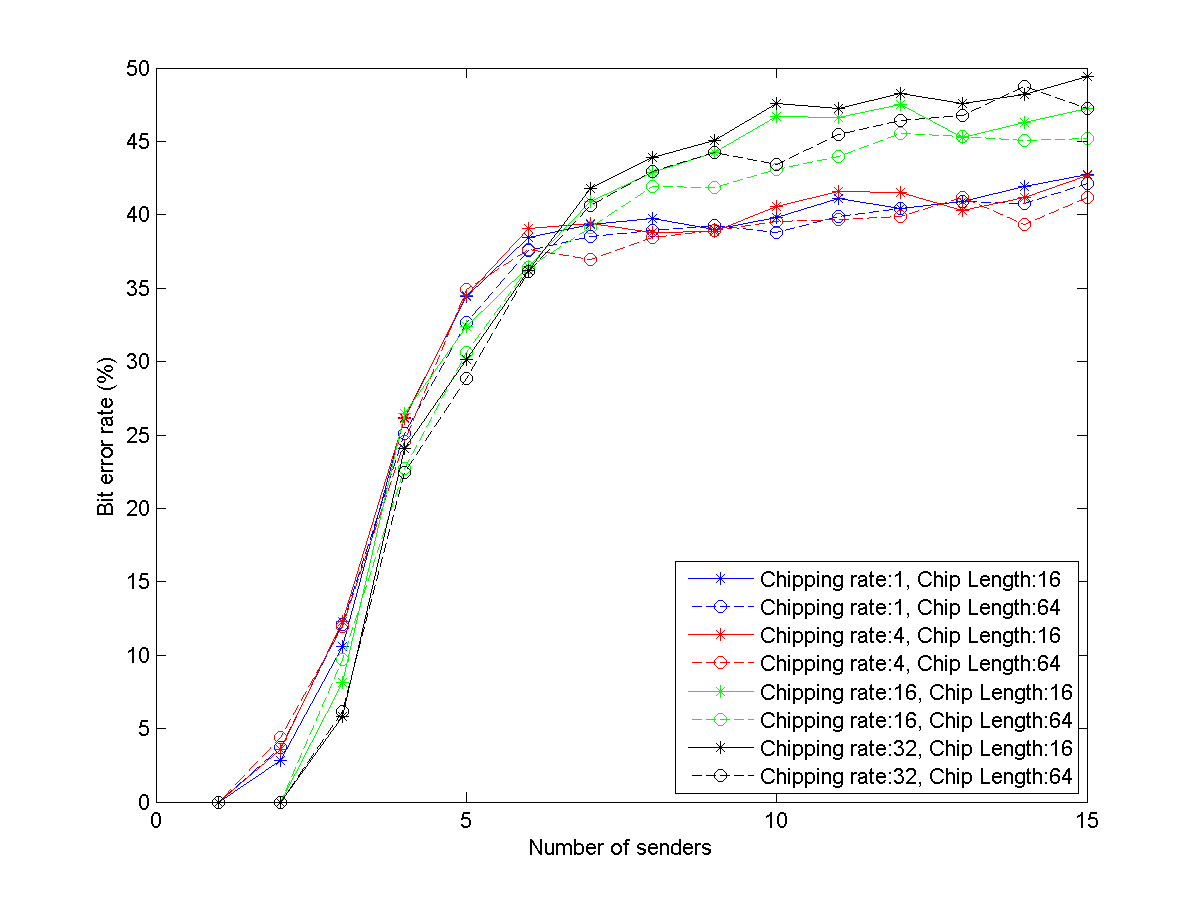
\includegraphics[width=0.5\textwidth]{imgs/results/plot_mode_fhss-test_numSenders-rep_20-dataRate_8-dataLength_128.png}
				\caption{Multiuser}
				\label{fig:fhss_multiuser}
			\end{figure}
\section{Conclusion}
    
    
    Due to the different bandwidths both techniques use, a direct comparison is not straightforward. We can, however, state that DSSS reaches the same performance in multiuser scenarios as our FHSS implementation while using a chipping rate of 16, which means a bandwidth of 32 Hz, where FHSS employed 1024 Hz. Our DSSS implementation also performed better in our "real-life noise" test and was more robust to Gaussian noise. FHSS, however, performed better in narrowband interference test scenario and is more practical to scale up to more users.
    
    In conclusion, we should have rediscussed using FSK for fast-hopping FHSS, as we think we could not properly show the potential of this technique.
    
    
    Further work could include support for simulation of free-space path loss. The distance between the sender and the receiver would then influence the quality of the signal. Additionally we could extend the free-space path loss by using a custom propagation coefficient to simulate more complex environments like buildings and other obstacles that prevent direct line of sight.
    
    
    Another project could be to not only measure bit-error rates, but also introduce a packet-error rate. To support this we would first need to decide how a packet should be defined. One possibility would be to combine a fixed amount of bits to a packet or send a special bit sequence to announce the beginning of a new packet.


%The bibliography, done here without a bib file
%This is the old BibTeX style for use with llncs.cls
\bibliographystyle{splncs}

%Alternative bibliography styles:
%the following does the same as above except with alphabetic sorting
%\bibliographystyle{splncs_srt}
%the following is the current LNCS BibTex with alphabetic sorting
%\bibliographystyle{splncs03}
%If you want to use a different BibTex style include [oribibl] in the document class line

\begin{thebibliography}{1}
%add each reference in here like this:
\bibitem[ISS]{ISS}
Author: Jan De Nayerlaan
Article: Spread Spectrum
Year: (1999) 
\bibitem[wirelesscommunication.nl]{web-nl}
Glas, Jack. "Frequency Hopping." Frequency Hopping. Wirelesscommunication.nl, n.d. Web. 07 Dec. 2014. http://www.wirelesscommunication.nl/reference/chaptr05/spreadsp/fh.htm
\end{thebibliography}




\end{document}

